\section{Practical Gradient Boosted Regression}
%
\begin{frame}[fragile]
Scikit-learn includes the gradient boosted regression algorithm in the \texttt{ensembles} module\\~\\

\begin{lstlisting}[language=python]
from sklearn.ensemble import GradientBoostedRegressor
\end{lstlisting}

\end{frame}
%
\begin{frame}[fragile]

\texttt{GradientBoostingRegressor} has many knobs to turn.\\~\\

\begin{lstlisting}[language=python]
GradientBoostingRegressor(loss='ls', 
                          learning_rate=0.1, 
                          n_estimators=100, 
                          subsample=1.0, 
                          min_samples_split=2, 
                          min_samples_leaf=1, 
                          min_weight_fraction_leaf=0.0,
                          max_depth=3,
                          ...)
\end{lstlisting}

\end{frame}
%
\begin{frame}[fragile]
A \texttt{GradientBoostingRegressor} object is fit in the same way as every other leaning model in sklearn\\~\\

\begin{lstlisting}[language=python]
model = GradientBoostingRegressor()
model.fit(X, y)
\end{lstlisting}

\end{frame}
%
\begin{frame}[fragile]
The \texttt{predict} method returns predictions on new data\\~\\

\begin{lstlisting}[language=python]
preds = model.predict(X_new)
\end{lstlisting}

Especially useful is the iterator \texttt{staged\_predict} which creates predictions from models created by truncating series of trees\\~\\

\begin{lstlisting}[language=python]
for preds in model.staged_predict(X_new):
    # Do something interesting, see the plots below.
\end{lstlisting}

\end{frame}
%
\begin{frame}[fragile]
The most important options to \texttt{GradientBoostedRegressor} are

\begin{itemize}
  \item \texttt{loss} controls the loss function to minimize.  \texttt{ls} is the least squares minimization algorithm we discussed in the previous section.
  \item \texttt{n\_estiamtors} is how many boosting stages to compute, i.e. how many regression trees to grow.
  \item \texttt{learning\_rate} is the learning rate for the gradient update.
  \item \texttt{max\_depth} controls how deep to grow each individual tree.
  \item \texttt{subsample} allows to fit each tree on a random sample of the training data (like bagging in random forests).
\end{itemize}

\end{frame}
%
\begin{frame}{Tuning the Number of Estimators}

As more and more trees are added to the model the training set error will be driven down monotonically, but the same is not true for the testing error

  \begin{figure}
    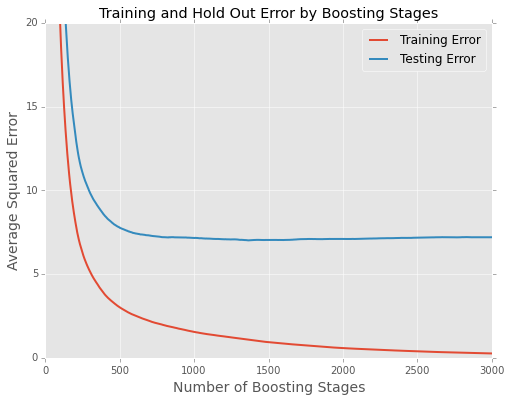
\includegraphics[scale=0.45]{training-and-testing-error}
  \end{figure}

\end{frame}
%
\begin{frame}

  \begin{figure}
    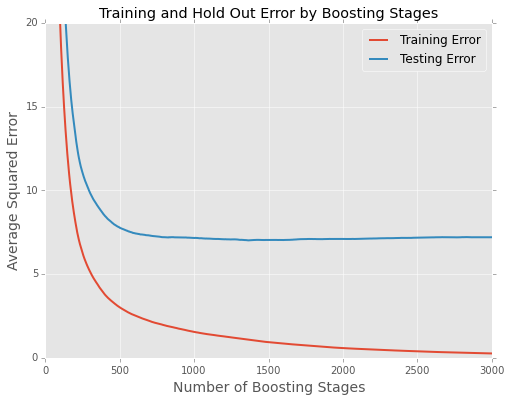
\includegraphics[scale=0.45]{training-and-testing-error}
  \end{figure}

This means that it is essential to determine the proper number of trees to grow, as too many may lead to overfitting

\end{frame}
%
\begin{frame}
One way to tune the numer of trees is to make use of a validation set, held out from both training and testing

  \begin{figure}
    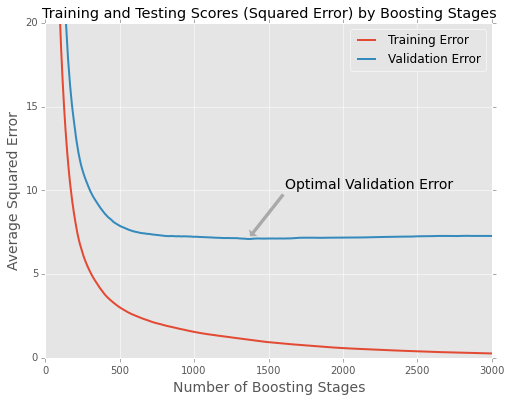
\includegraphics[scale=0.45]{training-and-testing-error-with-optima}
  \end{figure}
  
\end{frame}
%
\begin{frame}[fragile]
The \texttt{loss\_} method is important here, it allows us to compute the loss function on held out data\\~\\

\begin{lstlisting}[language=python]
validation_loss = np.zeros(model.get_params('n_estimators'))
for i, preds in enumerate(model.staged_predict(X_new)):
    validation_loss[i] = model.loss_(preds, y_new)
    
optimal_tree = np.argmin(validation_loss)
optimal_loss = validation_loss[optimal_tree]
\end{lstlisting}

\end{frame}
%
\begin{frame}
Another way to choose the optimal number of trees is to replace the validation set with cross validation

  \begin{figure}
    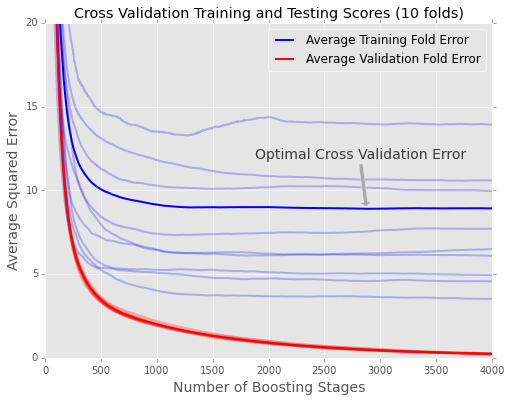
\includegraphics[scale=0.45]{training-and-testing-cv-error}
  \end{figure}
  
\end{frame}
%
\begin{frame}

  \begin{figure}
    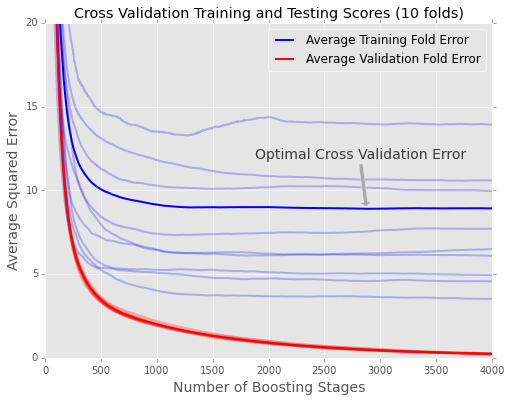
\includegraphics[scale=0.45]{training-and-testing-cv-error}
  \end{figure}
  
We generally choose the number of trees minimizing the \textit{average} out validation fold error.

\end{frame}
%
\begin{frame}{Tuning the Learning Rate}
In general, a smaller learning rate results in a more accurate model in the long run

  \begin{figure}
    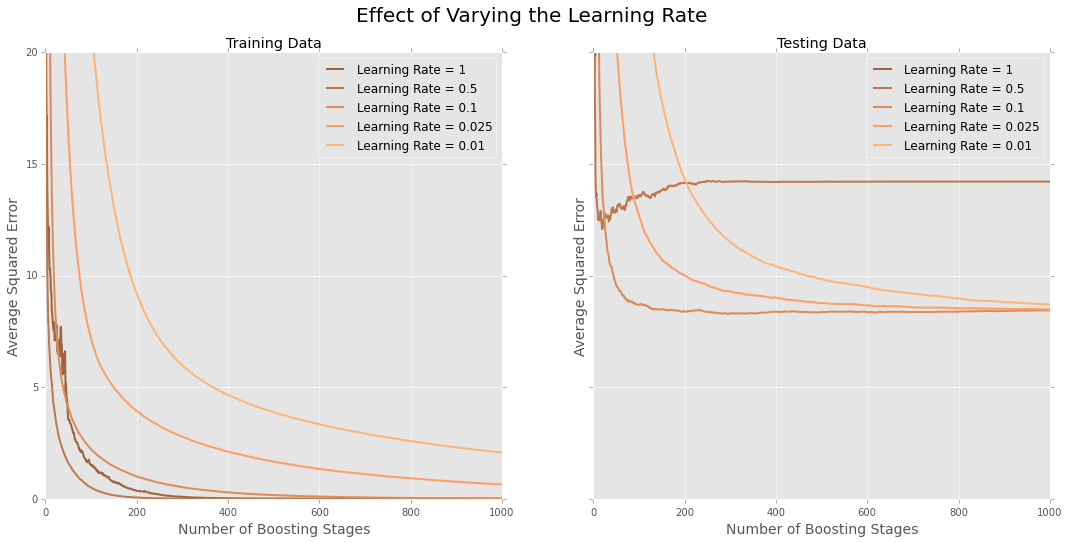
\includegraphics[scale=0.30]{varying-learning-rate-error}
  \end{figure}
  
\end{frame}
%
\begin{frame}
On the other hand, a smaller learning rate means more trees are needed to reach the optimal point

  \begin{figure}
    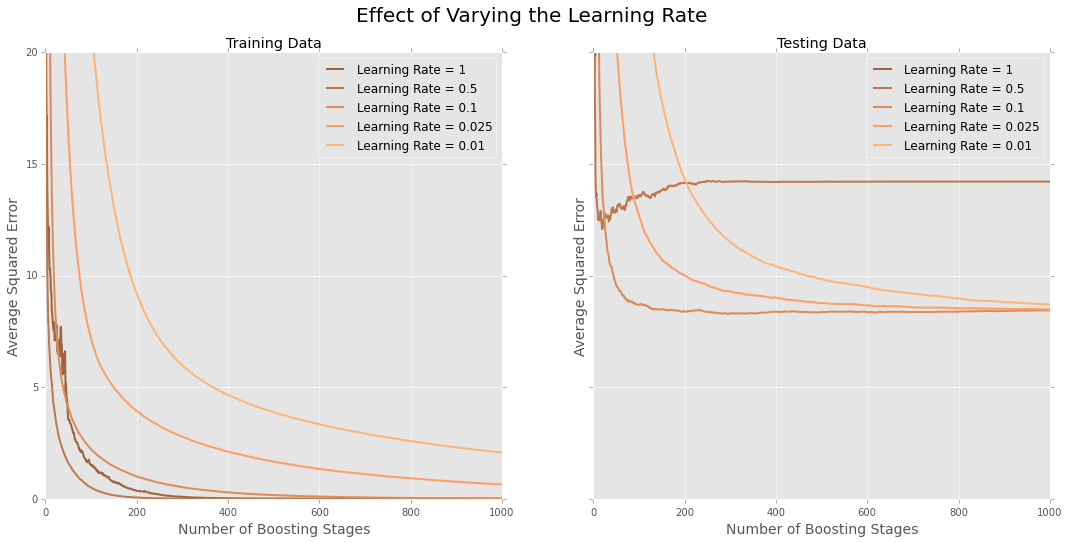
\includegraphics[scale=0.30]{varying-learning-rate-error}
  \end{figure}
  
\end{frame}
%
\begin{frame}
\textbf{Strategy for Learning Rate}:

\begin{itemize}
  \item In the initial exploratory phases of modeling, set the learning rate to some large value, say $0.1$.  This allows you to iterate through ideas quickly.
  \item When tuning other parameters using grid search, decrease the learning rate to a more sensible value, $0.01$ works well.
  \item When fitting the \textit{final} production model, set the learning rate to a very small value, $0.001$ or $0.0005$, smaller is better.
\end{itemize}

\end{frame}
%
\begin{frame}

Run the final model overnight!  It will fit while you are sleeping!\\~\\

Make sure you've written all your analysis code up front, based on your initial models.  Then all that's left is to run your final model through and see your final statistics.
\end{frame}
%
\begin{frame}{Tuning the Tree Depth}
A larger tree depth allows the model to capture deeper interactions between the predictors.

  \begin{figure}
    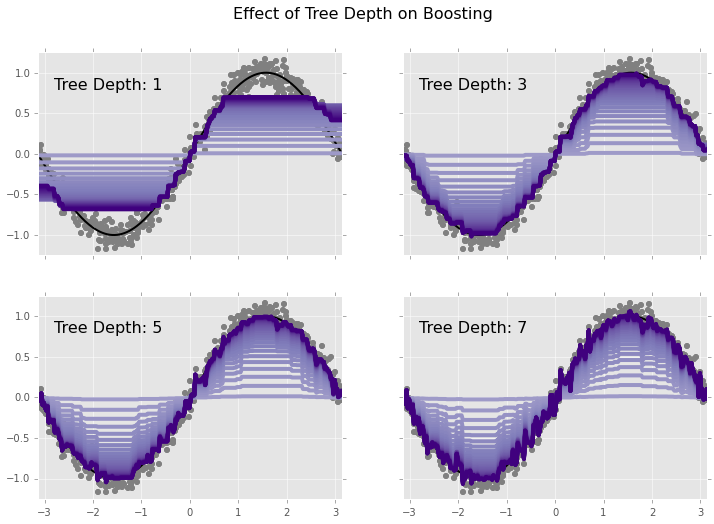
\includegraphics[scale=0.3]{sin-changing-depth}
  \end{figure}
  

Unfortunately, a deeper tree depth also causes the model to fit faster, somewhat combating the effect of the learning rate.
\end{frame}
%
\begin{frame}
It's never obvious up front what tree depth is best for a given problem, so a grid search is needed to determine the best value

  \begin{figure}
    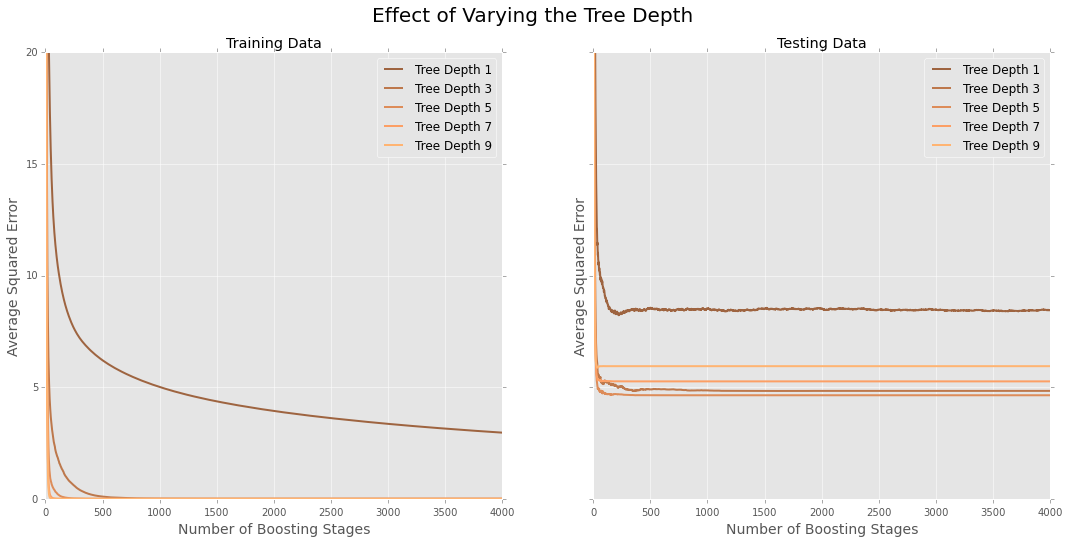
\includegraphics[scale=0.30]{varying-tree-depth-error}
  \end{figure}
  
\end{frame}


  